\documentclass{standalone}
\usepackage{tikz}
\usetikzlibrary{matrix,decorations.pathreplacing, calc, positioning,fit}
\begin{document}
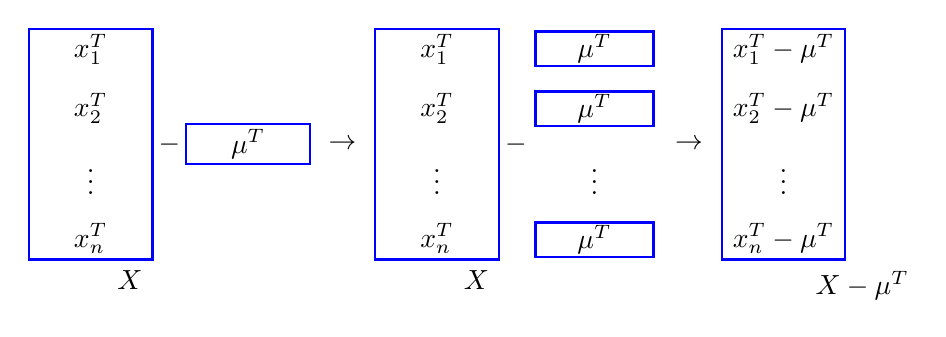
\begin{tikzpicture}[>=stealth,thick,baseline,
  mtxstyle/.style={
    matrix of nodes,
    draw=blue,
    minimum width=1.5cm,
    inner sep=1pt,
    row sep=3mm},
  vecstyle/.style={
    draw = blue,
    minimum width=1.5cm,
    inner sep=1pt}
    ]
% \tikzstyle{mxborder} = [matrix of mathnodes, draw, blue];
    \matrix (A) [mtxstyle] {
    $x_{1}^T$\\
    $x_{2}^T$\\
    $\vdots$\\
    $x_{n}^T$\\
   };
   \node (Ax) [right=0.5cm of A.south, anchor=north] {$X$};
   \node (B) [right of = A] {$-$};
   \node (C) [right of = B, mtxstyle] {
   $\mu^T$\\
   };
   \node (D) [right of = C, xshift=2mm] {$\rightarrow$};
    \matrix (E) [mtxstyle, right of=D, xshift=2mm] {
    {$x_{1}^T$}\\
    {$x_{2}^T$}\\
    $\vdots$\\
    {$x_{n}^T$}\\
   };
  \node (Ex) [right=0.5cm of E.south, anchor=north] {$X$};
   \node (F) [right of = E] {$-$};
    \matrix (G) [mtxstyle, draw=none, right of= F] {
    \node [vecstyle] {$\mu^T$};\\
    \node [vecstyle] {$\mu^T$};\\
    $\vdots$\\
    \node [vecstyle] {$\mu^T$};\\
   };
   \node (H) [right of = G, xshift=2mm] {$\rightarrow$};
    \matrix (I) [mtxstyle, right of=H, xshift=2mm] {
      {$x_{1}^T - \mu^T$}\\
      {$x_{2}^T - \mu^T$}\\
    $\vdots$\\
      {$x_{n}^T - \mu^T$}\\
   };
  \node (Ix) [right=1cm of I.south, anchor=north] {$X - \mu^T$};

\end{tikzpicture}
\end{document}